\documentclass[a4paper]{article}

\usepackage[T1]{fontenc}
\usepackage[utf8]{inputenc}
\usepackage[english]{babel}
\usepackage{eurosym}
\usepackage{setspace}
\usepackage{tikz}
\usepackage{pgf-umlcd}
\usepackage{pgf-umlsd}
\usepackage{hyperref}
\hypersetup{
    colorlinks=true,
    linkcolor=black,
    filecolor=black,
    urlcolor=black,
}
\usepackage{amssymb}
\usepackage{amsthm}
\usepackage{mathtools}
\usepackage{bm}



\textwidth=450pt
\oddsidemargin=0pt
\textheight=665pt
\voffset=-50pt

\singlespacing

\begin{document}

\begin{titlepage}
	\begin{center}
		
\includegraphics[height=5cm]{minerva.pdf}

		\vspace*{1.75cm}

		\LARGE

		\textbf{MSc in Computer Science} \\
		at University of Milan

		\vspace*{1cm}

		\huge
		CHIP-8 STM32

		\large Proposta per il Progetto di PROS, \\
		corso tenuto da \textbf{Danilo Bruschi}

		\normalsize
		\vspace*{4cm}

		\begin{minipage}[t]{0.47\textwidth}
			{Email: } \vspace{0.3em} \\
			{\large \href{federico.bruzzone@studenti.unimi.it}{federico.bruzzone@studenti.unimi.it}} \vspace{1em}  \\
			{\large \href{lorenzo.ferrante1@studenti.unimi.it}{lorenzo.ferrante1@studenti.unimi.it}} \vspace{1em}  \\
			{\large \href{andrea.longoni3@studenti.unimi.it}{andrea.longoni3@studenti.unimi.it}} \vspace{1em}  \\
		\end{minipage}
		\hfill
		\begin{minipage}[t]{0.47\textwidth}\raggedleft
			{Creato da:} \hspace{-0.9em} \vspace{0.3em} \\
			{\large \textbf{Federico Bruzzone}} \\
			\vspace{1em}
			{\large \textbf{Lorenzo Ferrante}} \\
			\vspace{1em}
			{\large \textbf{Andrea Longoni}}
		\end{minipage}

		\vfill
		Anno accademico 2022/2023

	\end{center}
\end{titlepage}

\setlength{\parindent}{0pt}
\setlength{\parskip}{0.8em}
\linespread{1.5}

\section{Introduzione}

CHIP-8 é un linguaggio di programmazione creato a metà degli anni '70 da Joseph Weisbecker per semplificare lo sviluppo di videogiochi per microcomputer a 8 bit. I programmi CHIP-8 vengono interpretati da una macchina virtuale che é stata estesa parecchie volte nel corso degli anni, tra le versioni più adottate citiamo S-CHIP e la più recente XO-CHIP.

La semplicità dell'interprete in aggiunta alla sua lunga storia e popolarità hanno fatto sì che emulatori e programmi CHIP-8 vengano realizzati ancora oggi. Nel corso degli anni molti videogiochi storici sono stati "portati" su CHIP-8 tra cui Pong, Space Invaders e Tetris.

Lo scopo del progetto é quello di costruire un emulatore CHIP-8 e S-CHIP in grado di funzionare su un microcontrollore STM32.

\section{Analisi di Mercato}

Al giorno d'oggi risulta difficile ottenere un numero esatto di utenti, ma possiamo basarci sul topic "chip8" di GitHub che raggruppa quasi un migliaio di repository.

Tra queste la più popolare è Octo, un'implementazione scritta in JavaScript capace di eseguire la versione base di CHIP-8, S-CHIP e XO-CHIP nel browser. La repository è mantenuta da John Earnest, l'inventore di XO-CHIP che nel 2014 ha riportato in vita CHIP-8 modernizzandolo e aggiungendo nuove funzionalità.

Inoltre ogni anno viene organizzata la Octojam, una game jam dove ogni partecipante prova a sviluppare un videogioco per CHIP-8 (o per le sue estensioni) partendo da zero.

Grazie al suo instruction set ridotto e alla sua limitata richiesta di risorse hardware è stato portato su un elevato numero di piattaforme, tra cui il Game Boy Color, calcolatrici grafiche serie HP 48 e Emacs (il famoso editor di testo).

Sebbene CHIP-8 e S-CHIP siano stati tradizionalmente implementati tramite software esistono anche implementazioni hardware. Ne citiamo una in particolare scritta nel linguaggio Verilog per schede FPGA.

\section{Componenti Hardware}

% 4 Kb per ROM + 4 Kb per VM

% Abbiamo deciso di utilizzare questa scheda perché le ROM dei giochi CHIP-8 e S-CHIP che devono essere caricati in SRAM hanno dimensione massima di 4 \texttt{Kb}. Questa quantità aggiunta ai 4kb di ram emulata del computer originale del chip 8 ci fa capire di aver bisogno di più di 8kb di SRAM. 16 Kb dovrebbe bastare lasciandoci spazio per 8kb di codice

Il componente principale é il microcontrollore \texttt{STM32F334R8T6} basato su architettura ARM con processore Cortex-M4 da 72 \texttt{MHz}, 64 \texttt{Kb} di memoria flash e 16 \texttt{Kb} di SRAM. Abbiamo deciso di utilizzare questa scheda perché le ROM dei giochi CHIP-8 e S-CHIP hanno dimensione massima di 4 \texttt{Kb}. Considerando questo e il fatto che la macchina virtuale necessita 4 Kb per poter funzionare non è stato potuto utilizzare la scheda fornitaci durante il corso a causa della sua quantità limita di SRAM.

Necessiteremo inoltre di un display TFT LCD (thin-film-transistor liquid-crystal display) a colori retroilluminato, per poterci interfacciare col gioco. Questo display, da 2.4 pollici, é basato sul controller \texttt{ILI9341} e ha una risoluzione di 320$\times$240 \texttt{px}.

Il display dispone di un lettore di schede microSD, che verrà utilizzato per caricare una delle ROM presenti sulla SD in SRAM.

Per interagire con l'emulatore utilizzeremo una tastiera matriciale 4$\times$4 corrispondente alla tastiera esadecimale originale.

Per riprodurre gli effetti sonori generati dal gioco utilizzeremo un beeper a frequenza variabile. In CHIP-8 e S-CHIP vi é un solo tipo di suono che può essere riprodotto durante tutta l'esecuzione del gioco. Infine sarà possibile aggiungere uno slot per l'alimentazione tramite due batterie \texttt{AA}.

\section{Componenti Software}

Le parti software che saranno implementate sono:

\begin{enumerate}
	\item La \textbf{Macchina Virtuale} (VM) che interpreta programmi CHIP-8 e S-CHIP. Non volendoci affidare ad implementazioni già esistenti abbiamo deciso di svilupparla da zero, per questo motivo verrà effettuato il testing con un'interfaccia emulata su un calcolatore \textrm{x}86 a 64 \texttt{bit} tramite SDL2 o Raylib (due librerie per creare interfacce multimediali in C). Successivamente verrà portata sul microcontrollore basato su ARM Cortex-M.
	\item Il \textbf{Driver Video} che permette l'interfacciamento tra il microcontrollore e il display TFT LCD. Lo schermo supporta interfacce parallele a 8 \texttt{bit} e SPI a 4 pin, per ragioni di prestazioni noi implementeremo il driver utilizzando l'interfaccia parallela a 8 \texttt{bit}.
	\item Il \textbf{Driver microSD} che permette l'interfacciamento tra il microcontrollore e il lettore della scheda SD, verrà sviluppato utilizzando l'interfaccia SPI. Per questo driver utilizzeremo le librerie fornite da ST per la gestione del filesystem \texttt{FAT32} e facilitare lo sviluppo del trasferimento dati.
	\item Il \textbf{Driver Keypad} che permette l'interfacciamento tra il microcontrollore e la tastiera matriciale 4$\times$4. La gestione degli input da tastiera non verrà effettuata in polling, ma bens\'{i} tramite interrupt.
	\item Il \textbf{Driver Sound} che permette l'interfacciamento tra il microcontrollore e il beeper. Il driver permette di generare suoni a frequenza variabile.
\end{enumerate}

Inoltre verrà implementato un menù per la selezione del gioco all'avvio dell'emulatore. Infine abbiamo deciso di non usare librerie esterne ma di sviluppare una nostra libreria per effettuare il rendering del font e disegnare sul display.

\section{Architettura Software}

\subsection{Class Diagram}

\renewcommand{\umltextcolor}{black}
\renewcommand{\umldrawcolor}{black}
\renewcommand{\umlfillcolor}{white}
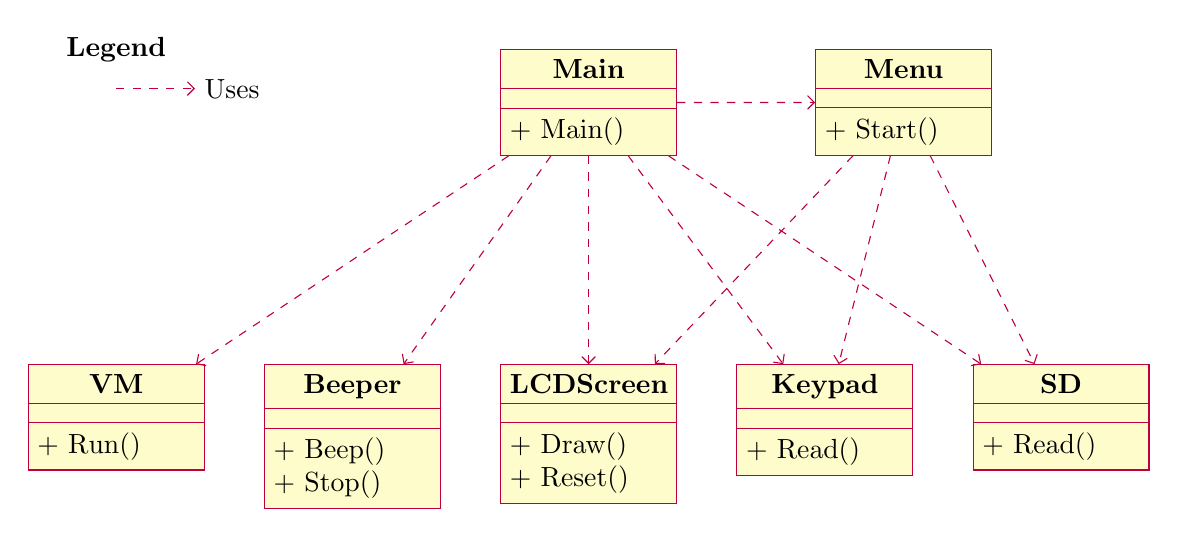
\begin{tikzpicture}
  \begin{class}[text width=2cm]{Main}{6,0}
    \operation{+ Main()}
  \end{class}

  \begin{class}[text width=2cm]{Menu}{10,0}
    \operation{+ Start()}
  \end{class}

  \begin{class}[text width=2cm]{VM}{0,-4}
    \operation{+ Run()}
  \end{class}

  \begin{class}[text width=2cm]{Beeper}{3,-4}
    \operation{+ Beep()}
    \operation{+ Stop()}
  \end{class}
  
  \begin{class}[text width=2cm]{LCDScreen}{6, -4}
    \operation{+ Draw()}
    \operation{+ Reset()}
  \end{class}

  \begin{class}[text width=2cm]{Keypad}{9,-4}
    \operation{+ Read()}
  \end{class}
  
  \begin{class}[text width=2cm]{SD}{12, -4}
    \operation{+ Read()}
  \end{class}

    \draw [umlcd style dashed line , ->] (Menu) -- node [ above , sloped , black ]{} (Keypad) ;
    \draw [umlcd style dashed line , ->] (Menu) -- node [ above , sloped , black ]{} (SD) ;
    \draw [umlcd style dashed line , fill=white, ->] (Menu) -- node [ below  , black ]{} (LCDScreen) ;

    \draw [umlcd style dashed line , ->] (Main) -- node [ above , sloped , black ]{} (Menu) ;
    \draw [umlcd style dashed line , ->] (Main) -- node [ above , sloped , black ]{} (VM) ;
    \draw [umlcd style dashed line , ->] (Main) -- node [ above , sloped , black ]{} (Keypad) ;
    \draw [umlcd style dashed line , ->] (Main) -- node [ above , sloped , black ]{} (Beeper) ;
    \draw [umlcd style dashed line , fill=white, ->] (Main) -- node [ below , sloped , black ]{} (SD) ;
    \draw [umlcd style dashed line , fill=white, ->] (Main) -- node [ below , sloped , black ]{} (LCDScreen) ;

    \begin{scope}[xshift=0cm, yshift=0cm] % Adjust the positioning of the legend
    % Legend title
    \node[font=\bfseries] at (0, 0) {Legend};
    % Legend items
    \draw [umlcd style dashed line , fill=white, ->] (0, -0.5) -- (1, -0.5) node[right,  black] {Uses};
    \end{scope}

  % \draw [ umlcd style , ->] (Main) -- node [ above , sloped , black ]{$ < <$ import $ > >$} (Student) ;
\end{tikzpicture}

\subsection{Sequence Diagram}

\begin{figure}[!htbp]
    \centering
    \resizebox{1\textwidth}{!}{%
        \begin{sequencediagram}
        \newthread{main}{:Main}
        \newinst[0.5]{menu}{:Menu}
        \newinst[0.5]{vm}{:VM}
        \newinst[0.5]{lcd}{:LCD}
        \newinst[0.5]{kp}{:Keypad}
        \newinst[0.5]{beep}{:Beeper}
        \newinst[0.5]{sd}{:SD}

        \begin{call}{main}{Menu\_Start()}{menu}{}
            \begin{call}{menu}{SD\_GetGames()}{sd}{}
            \end{call}
            \begin{sdblock}{ChooseGameLoop}{}
                \begin{call}{menu}{Keypad\_PressKey()}{kp}{}
                \end{call}
                \begin{call}{menu}{LCD\_DrawMenu()}{lcd}{}
                \end{call}
            \end{sdblock}
            \begin{call}{menu}{SD\_LoadGame()}{sd}{}
            \end{call}
        \end{call}

        \begin{sdblock}{MainLoop}{}
            \begin{call}{main}{KP\_PressKey()}{kp}{}
            \end{call}
            \begin{call}{main}{VM\_StepCpu()}{vm}{}
            \end{call}
            \begin{call}{main}{Beeper\_Beep()}{beep}{}
            \end{call}
            \begin{call}{main}{LCD\_Draw()}{lcd}{}
            \end{call}
        \end{sdblock}
        \end{sequencediagram}
    }
\end{figure}

\section{Analisi del Consumo Energetico}

Come abbiamo gi\'a accennato in precedenza il microcontrollore durante lo sviluppo verrà alimentato tramite USB e successivamente utilizzando batterie \texttt{AA}. Le batterie hanno una tensione di 3\texttt{V} e una capacit\'a di $\sim$2500 \texttt{mA} e usandone due in serie otterremo 5000 \texttt{mA}.

Stimando un consumo dello schermo di 100 \texttt{mAh} e un consumo di 25 \texttt{mAh} per il microcontrollore e le sue periferiche, avremo un consumo totale di 125 \texttt{mAh}.

\begin{equation*}
    \begin{aligned}
        \textmd{time} \ (\texttt{h}) & = \frac{\textmd{capacity} \ (\texttt{mA})}{\textmd{consumption} \ (\texttt{mAh})}\\
                                     & = \frac{2 * 2500 \ \texttt{mA}}{125 \ \texttt{mAh}}\\
                                     & = 40 \ \texttt{h}
    \end{aligned}
\end{equation*}

Possiamo stimare una durata di 40 ore di gioco.

\section{Analisi di Tempi e Costi}

\begin{center}
	\begin{table}[ht]
		\centering
		\begin{tabular}{|llll|l|}
			\hline
			\multicolumn{1}{|l|}{\textbf{Nome}}                   & \multicolumn{1}{l|}{\textbf{Modello}}       & \multicolumn{1}{l|}{\textbf{Costo unitario}} & \textbf{Unità} & \textbf{Costo} \\ \hline
			\multicolumn{1}{|l|}{Schermo}                & \multicolumn{1}{l|}{ILI9341 2.4"}           & \multicolumn{1}{l|}{6.44}                    & 1               & 6.50           \\ \hline
			\multicolumn{1}{|l|}{Matrix keypad}          & \multicolumn{1}{l|}{AZ-Delivery 4$\times$4}        & \multicolumn{1}{l|}{3.99}                    & 1               & 3.99           \\ \hline
			\multicolumn{1}{|l|}{Microcontrollore}       & \multicolumn{1}{l|}{STM32 F334R8T6}         & \multicolumn{1}{l|}{14.99}                   & 1               & 14.99          \\ \hline
			\multicolumn{1}{|l|}{Beeper}                 & \multicolumn{1}{l|}{}                       & \multicolumn{1}{l|}{0.99}                    & 1               & 0.99           \\ \hline
			\multicolumn{1}{|l|}{Breadboard e cablaggio} & \multicolumn{1}{l|}{}                       & \multicolumn{1}{l|}{4.99}                    & 1               & 4.99           \\ \hline
			\multicolumn{4}{|r|}{\textbf{Totale}}                                                                                                            & 31.50\euro        \\ \hline
		\end{tabular}
		\caption{
			Materiali previsti per la costruzione del progetto. I costi indicati
			provengono da negozi online come Amazon e eBay
		}
	\end{table}
\end{center}

\begin{center}
	\begin{table}[ht]
		\centering
		\begin{tabular}{|l|l|}
			\hline
			\textbf{Nome}                         & \textbf{Tempo di lavoro} \\ \hline
			Macchina virtuale                     & 3 settimane              \\ \hline
			Driver video                          & 1 settimana              \\ \hline
			Driver microSD                        & 3 giorni                 \\ \hline
			Driver keypad                         & 1 giorno                 \\ \hline
			Driver audio                          & 5 giorni                 \\ \hline
			Selezione gioco                       & 5 giorni                 \\ \hline
			Ottimizzazione software               & 2 settimane              \\ \hline
			\multicolumn{1}{|r|}{\textbf{Totale}} & 2 mesi                   \\ \hline
		\end{tabular}
		\caption{
			Tempi previsti per la realizzazione dei componenti software
		}
	\end{table}

\end{center}

\end{document}
